\documentclass[article,english]{template/ample}

% used for example text
\usepackage{blindtext}
\renewcommand{\blindmarkup}[1]{\emph{#1}}

% document metadata
\title{The \emph{ample} template}
\author{Jesse Stricker}

% bibliography
\addbibresource{root.bib}

\begin{document}

\maketitle
\tableofcontents

% ==============================================================================

\section{Introduction}

Hello, \LaTeX.

\section{Localization}

Use can use \q{quotation marks} like this and \q{even \q{like} this}.

\section{Citations}

This is an example citation\cite{gunn2019}.

\section{Font test}

Show the main font, the \textsf{sans-serif} font and the \texttt{typewriter}
font.

\subsection{Main font}

\blindtext{}

\subsection{Sans-serif font}

{\sffamily\blindtext{}}

\subsection{Typewriter font}

\begin{listing}[H]
  \inputminted{rust}{assets/code-snippet.rs}
  \caption{A small Rust code snippet.\label{lst:small-rust}}
\end{listing}

\section{Units}

You can typeset angles like \ang{45}, numbers like \num{6.283}, units like
\unit{\kg\m\per\s\squared} and quantities like \qty{1.055e-34}{\J\s}.

\section{Tables}

\begin{table}[H]
  \centering
  \begin{tabular}{@{}cccS@{}} \toprule
    Header 1 & Header 2 & Header 3 & {Value} \\ \midrule
    Item 1,1 & Item 2,1 & Item 3,1 & 1.234   \\
    Item 1,2 & Item 2,2 & Item 3,2 & 12.45   \\ \bottomrule
  \end{tabular}
  \caption{A small table.\label{tab:small}}
\end{table}

\section{Math}

\begin{align}
  {(\vec{v} + \vec{w})}_i      & = \vec{v}_i + \vec{w}_i               \\
  {(\mat{M} + \mat{N})}_{ij}   & = {(\mat{M})}_{ij} + {(\mat{N})}_{ij} \\
  {(\ten{T} ⊗ \ten{U})}_{ijkl} & = \ten{T}_{ij} \cdot \ten{U}_{ij}
\end{align}

\begin{equation}
  z = 2\e^{(\tau/8)\i} = \sqrt{2} + \sqrt{2}\i
\end{equation}

\section{Graphics}

\begin{figure}[H]
  \centering
  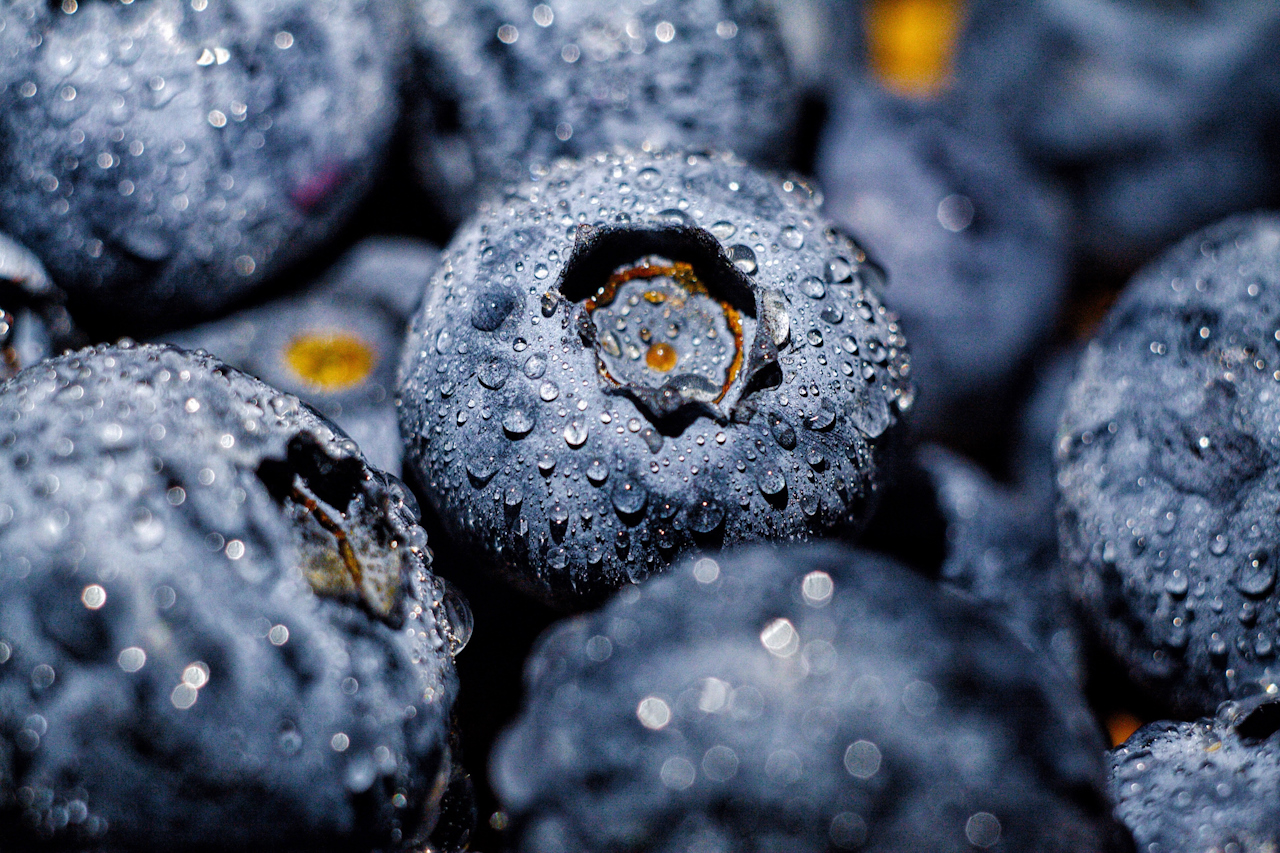
\includegraphics[width=\linewidth]{assets/pexels-dina-nasyrova-3628062.jpg}
  \caption{A close-up photo of blueberries.\label{fig:blueberries}}
\end{figure}

% ==============================================================================

\printbibliography{}

\end{document}
